\section{Sparse Matrices}
\label{introduction:sec:sparse}

Many problems, such as finite element and finite difference
discretizations~\cite{saad,duff} or problems arising from graph applications,
result in system matrices where the majority of elements are zero with
each row having only a few nonzero elements on average. Storing all these zeros
in an uncompressed, dense matrix is wasteful both in terms of storage and
computational cost, since the majority of the computations will be
multiplications or additions with zero. Furthermore, some of these systems
contain a very large number of unknowns (more than a million), so just storing
the matrix in double precision would exceed the memory capacity of a standard
computer server.

A common approach for dealing with such problems is to exploit the high fraction
of zeros in the matrix by storing only the nonzero elements, thus significantly
reducing the memory usage. In addition, if all operations that depend on the
matrix are implemented to directly use the compressed data, computational
savings can be obtained by skipping the operations involving zero elements
which are not stored.

\begin{figure}
\begin{subfigure}{\columnwidth}
\begin{center}
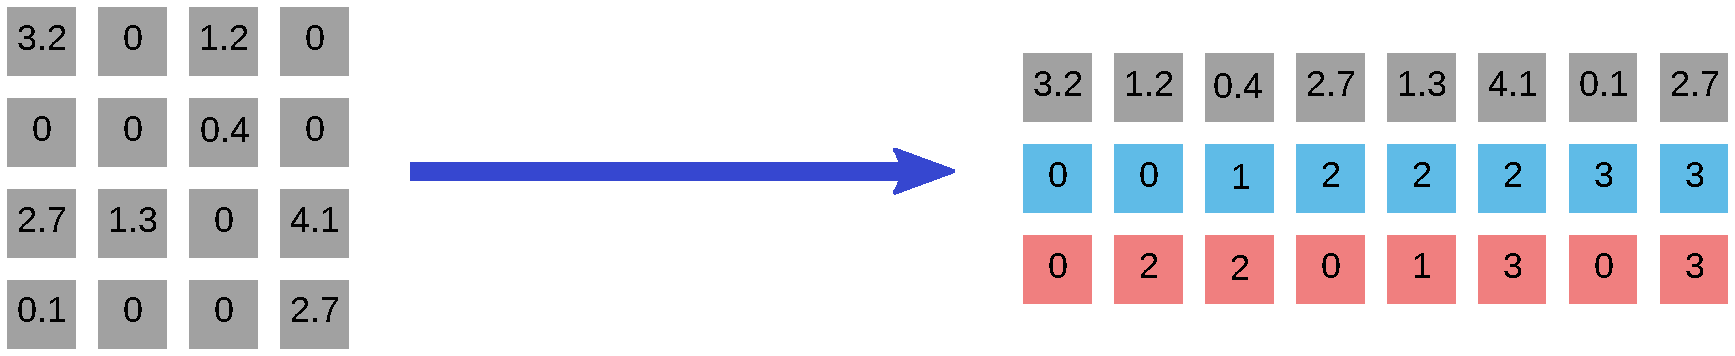
\includegraphics[width=.8\columnwidth]{plots/coo}
\end{center}
\caption{Coordinate format (COO)}
\end{subfigure} \\[2em]
\begin{subfigure}{\columnwidth}
\begin{center}
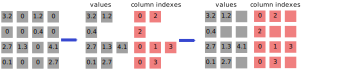
\includegraphics[width=.8\columnwidth]{plots/ell}
\end{center}
\caption{ELLPACK format (ELL)}
\end{subfigure} \\[2em]
\begin{subfigure}{\columnwidth}
\begin{center}
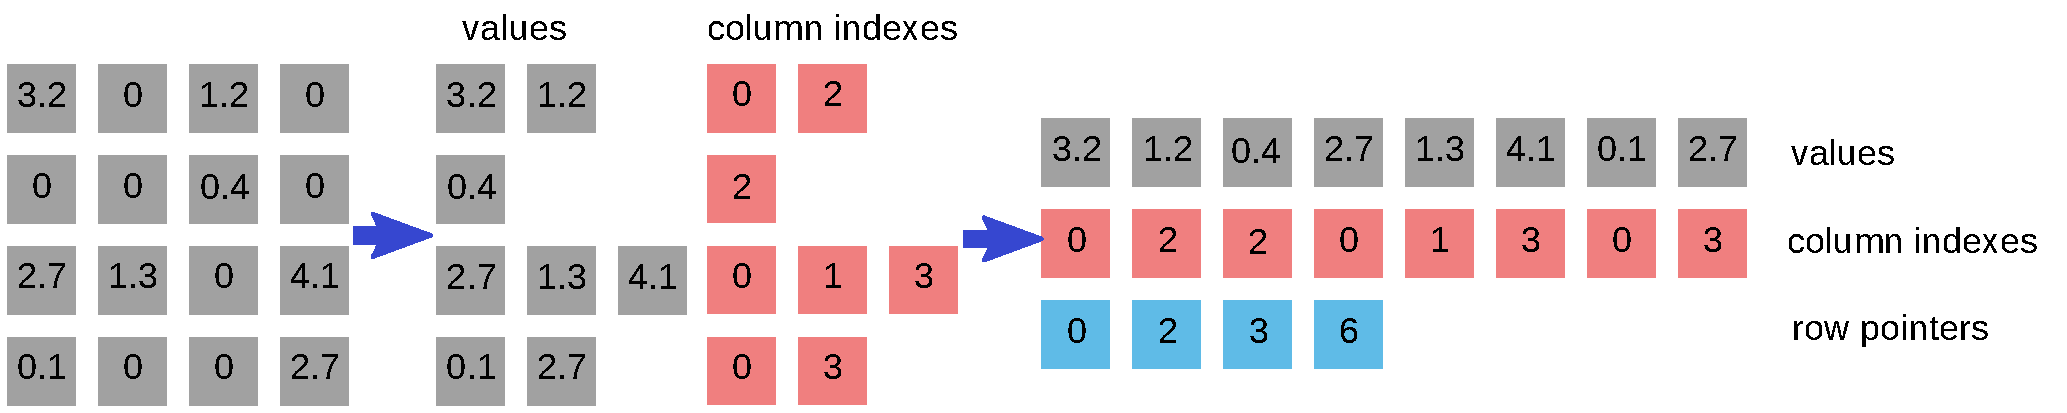
\includegraphics[width=.8\columnwidth]{plots/csr}
\end{center}
\caption{Compressed Sparse Row format (CSR)}
\end{subfigure}
\caption{Derivation of common sparse matrix storage formats.}
\label{introduction:fig:sparse-formats}
\end{figure}

Over the years, a variety of sparse matrix storage formats has been developed,
which aim at balancing the storage savings, and the efficient access of
stored data when performing the necessary operations. Derivation of the most
basic ones is shown graphically on Figure~\ref{introduction:fig:sparse-formats}.
The simplest one is the Coordinate format (COO). Its derivation is
straightforward: all nonzero entries are stored in sequence, and accompanied by
two indices which determine the position of that element in the matrix. The
information is stored in structure-of-arrays form --- a common approach when
storing sparse matrices so as to maximize cache efficiency. Another option is to
compress each row individually, only adding additional information about the
column index. The resulting data structure can then either be embedded into
square matrices by adding dummy elements as padding and storing them in one of
the dense matrix formats (usually in column-major order, that is column-by-column),
or individual rows can be stored in sequence and augmented with pointers to the
starting position of each row. This results in the so-called ELLPACK (ELL) and
Compressed Sparse Row (CSR) formats, respectively. Alternatively, one could
compress each column instead of each row, resulting in a column variant of
ELLPACK and the Compressed Sparse Column (CSC) format~\cite{saad}. In addition
to these basic formats, a number of advanced formats were developed to offer
additional memory and computational savings with certain algorithms,
applications, or on certain hardware. Common approaches include blocked versions
of basic formats~\cite{csb, bsr}, their various
combinations~\cite{sell-p,sell-c-sigma,bell-garland}, and their unconventional
enhancements~\cite{csr5, ecker}.

Even with a variety of available matrix formats, using them as part of method
implementations is nontrivial. In the context of direct methods, the first
challenge is the fact that factorizations do not preserve the sparsity pattern
(\ie the locations of nonzero elements) of the system matrix. Indeed, if the
system matrix contains a nonzero element on position $(i, j)$, the $L$
factor in the LU, Cholesky and LDL factorizations will generally have nonzeros
in all positions $(i, k)$ where $j \leq k \leq i$. Similarly, the $U$ factor in
LU factorizations will contain a nonzero in all positions $(k, j)$ where $i
\leq k \leq j$~\cite{duff}. A similar situation occurs with a matrix product
$AB$ of matrices $A$ and $B$ --- which is a common building block of QR
factorization algorithms~\cite{demmel} --- where $(AB)_{ij}$ is nonzero if there
exists an index $k$ such that both $A_{ik}$ and $B_{kj}$ are nonzero.
Consequently, depending on the sparsity pattern of the matrix, its
factorization may have a significantly larger proportion of nonzero elements, as
some positions that were zero in the original matrix become nonzero in the
factorized form (fill-in positions). To alleviate the problem, sparse direct
methods use various reordering (pivoting) strategies, such as the Reverse
Cuthill McKee (RCM), Minimum Degree (MD) and Nested Dissection (ND) orderings,
with the aim of moving the nonzeros closer to the diagonals and thus reducing
the amount of fill-in~\cite{saad, duff}. However, the strategies have to be
balanced with the preservation of numerical stability, and a good reordering is
not always easy to find, making the use of direct methods for sparse systems far
more limited than in the dense case~\cite{saad, duff}. An additional difficulty
is the fact that the exact amount and locations of the fill-in elements are
usually not known in advance, so sparse direct methods use several phases
\ha{two phases: symbolic phase and numeric phase}
\gf{Saad: ``\textit{
A typical sparse direct solution solver for positive definite matrices consists
of four phases. First, preordering is applied to reduce fill-in. Two popular
methods are used: minimum degree ordering and nested-dissection ordering.
Second, a symbolic factorization is performed. This means that the factorization
is processed only symbolically, i.e., without numerical values. Third, the
numerical factorization, in which the actual factors L and U are formed, is
processed. Finally, the forward and backward triangular sweeps are executed for
each different right-hand side. In a code where numerical pivoting is necessary,
the symbolic phase cannot be separated from the numerical factorization.''}
It's unclear what constitutes the ``factorization'' (preordering, symbolic fact.
and numeric fact., or just the factorizations), so I changed \textit{sparse
factorization methods} to \textit{sparse direct methods}, which does include
everything. It's definitely several phases, 4 or maybe less, and is not
necessary to specify exactly what is being done to understand the thesis. If
someone is interested in more details, they can look it up in Duff's book.}
\eq{:-)}
combined with specialized sparse storage formats that allow for the easy
insertion of new elements to the data structure~\cite{saad, duff}.

The situation is somewhat better in the case of iterative methods. Instead of
factorizing the matrix, relaxation methods split the matrix into the sum of two
matrices. In addition, the operation $y = M^{-1}Nx$ is usually calculated as a
matrix-vector product $z = Nx$, followed by a solution of the linear system $My
= z$, avoiding the need for inversions and matrix-matrix products which would
destroy the sparsity pattern.  Thus, the only operations required for relaxation
methods are the matrix-vector products with sparse matrices, solutions of linear
systems with sparse triangular or diagonal matrices, and the extraction of the
upper and lower triangles and the diagonals of the matrix from the sparse data
structure, which, at least for conventional storage formats, can usually be
realized by augmenting the sparse structure with pointers to the diagonal
elements. The only difficulty that occurs in both the relaxation methods, as
well as the solution step of direct methods, is the parallelization of
triangular system solves. While the operation is considered well-parallelizable
in the dense case, some sparsity structures make the operation hard to
parallelize, or even inherently sequential. An example of a matrix structure
that offers no parallelism whatsoever is the bidiagonal structure, which has
nonzero elements only on the main diagonal and the first diagonal below it. For
such a matrix, each stage of the forward substitution contains only one
operation. Furthermore, different stages cannot be parallelized, as each
subsequent stage depends on the result of the previous one.
In contrast to direct and relaxation methods, Krylov methods present the
ultimate solution when dealing with sparse matrices.  With the only requirement
being the matrix-vector product --- and in some cases the conjugate
matrix-vector product --- it is relatively simple to design a sparse matrix
format which allows computing this single operation efficiently. Even if the
format does not allow for efficient conjugate matrix-vector product, it is often
possible to explicitly store the conjugate transpose of the matrix in memory and
use the same algorithm as for the regular matrix-vector product.

In both direct and iterative methods, coming up with a single storage format for
all operations is extremely difficult. This is especially the case for highly
complicated and specialized formats, which are usually only designed to speed up
the matrix-vector product. Other operations are either not possible to realize
efficiently, or require significant implementation effort. Instead, most
software will rely on sometimes expensive format conversion procedures to
provide other operations when a specialized storage format is used. An
additional difficulty is interoperability between libraries, as every format
allows for slight variations of the basic scheme. As a result, the adoption of
specialized formats is extremely slow, with the majority of software packages
continuing to rely on basic storage
formats~\cite{ginkgo,paralution,vienna-cl,magma}. Among them, the CSR format is
considered the de-facto standard, as it usually offers the best storage
efficiency, and has historically provided the best performance on conventional
processor architectures.
